\section{Forward Kinematics [20 pts]}
For this exercise, you may use MATLAB or Python. Given the planar serial robot in Figure~\ref{fig:planar}, where each link is connected via a revolute (rotational) joint, except for the end-effector (the gripper), which is fixed to the final link:
% Insert image with caption
\begin{figure}[h!]
    \centering
    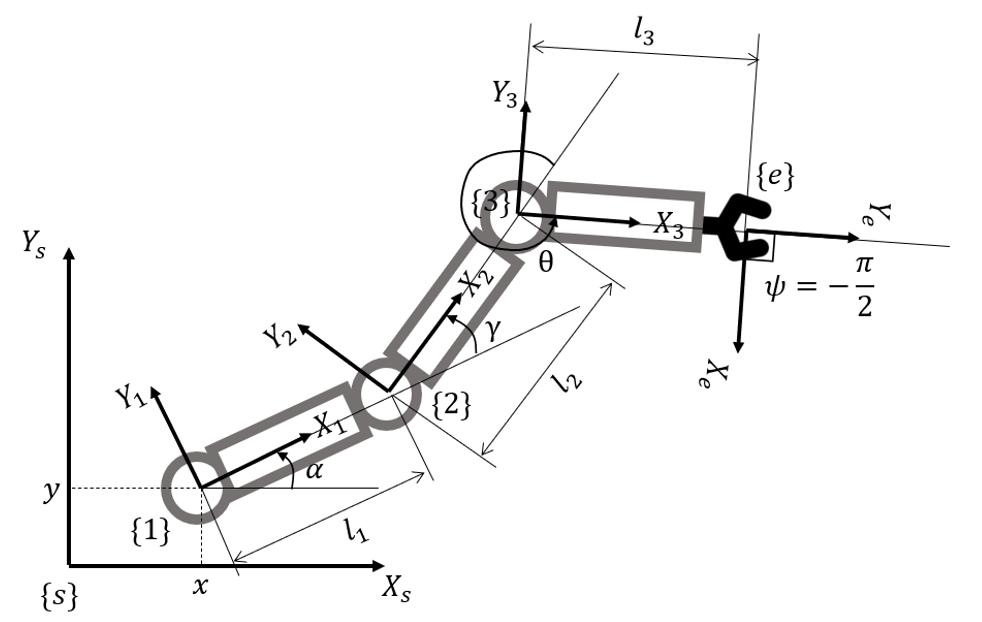
\includegraphics[width=0.7\textwidth]{img/planar.png}
    \caption{Planar serial manipulator}
    \label{fig:planar}
\end{figure}
\begin{enumerate}[(a)]  % (a), (b), (c), ...
\item Write the transformation matrices between subsequent reference frames, starting from the end-effector frame $\{e\}$ $(\mathbf{G}_e^3,\mathbf{G}_3^2,\dots,\mathbf{G}_1^s)$, and compute the transformation matrix from the end-effector frame $\{e\}$ to the global frame $\{s\}$. [10 pts]
\item At the following configuration of the robot:
\begin{equation*}
    \langle \alpha,\gamma,\theta\rangle=\langle \pi/4,\pi/4,-\pi/3\rangle, \quad l_1=l_2=l_3=1,\quad x=y=1
\end{equation*}
What are the coordinates of these point in the spatial frame $\{s\}$? $\mathbf{p}^e_1=\begin{bmatrix}
    0 \\0
\end{bmatrix}$, $\mathbf{p}^e_2=\begin{bmatrix}
    1 \\2
\end{bmatrix}$ [5 pts]
\item 	Suppose now that the robot base is fixed at $x=y=0$ (the origin of frame $\{1\}$ coincides with the origin of frame $\{s\}$), what is the expression of the velocity of a generic point $\mathbf{p}$ in the frame $\{2\}$ $(\mathbf{p}^2=\begin{bmatrix}
    x'\\y'
\end{bmatrix})$ with respect to the base frame $\{s\}$? Assume that the point $\mathbf{p}$ is rigidly fixed to frame $\{2\}$. Report the procedure and the final coordinates, no need to report the full symbolic equations at each step. [5 pts.]
\end{enumerate}